\section{Basic Concepts}
\label{sec:Basic-Concepts}

EXIP is a C library written in a portable manner that implements the EXI format for
XML representation. Probably a better way of describing what is EXIP is to say what it is \emph{not}.
EXIP is not a tool for converting text XML documents to EXI and vice versa. Why is that then?
To start with, the XML to EXI conversion requires a XML parser that process the XML input.
The XML parser itself is at least as big chunk of code as it is the EXI parser and having them
both at the same time might not be
possible or desired on a resource constrained embedded system. Second, parsing
the text XML and then converting it to EXI effectively removes all the processing benefits of EXI.
Having said that, it does not mean that it is not possible to use EXIP in such scenario. For example,
it is planned as a future work to include a module in EXIP that performs exactly that: generating
corresponding EXI streams from a text XML input and vice versa. It is therefore an optional
behavior and not an only possible way of using the library. It is not even difficult to implement
such a module and the reader could do that as a practical exercise after going through this guide.

As a result of this design choice, EXIP cannot use (at least for now) the XML Schema format directly
to perform schema-enabled processing. This might sound as a big flaw in the implementation but is
just the opposite. XML Schema documents are plain XML documents and as such they have analogous EXI
representation. Working with the EXI representation of the XML Schema definitions brings all the
performance benefits of the EXI itself - faster processing and more compact representation.
Now, using static systems where the schema information is only processed at design time would
not make much difference. However, once you are faced with more dynamic systems that are
capable of handling schema information at run-time, the use of EXI representation is more
beneficial especially in networked embedded environments.

Yet another \emph{not} - EXIP is not compliant with DOM, SAX or StAX Application Programming Interfaces (APIs)
for XML processing. The single reason for that is the efficiency trade-off. All these APIs are
using string representation of the primitive data types defined by the XML Schema specification
such as float, integer, date etc. This means that when schema definitions are available these
types must be converted from native types to string and then back from string to native representation
in order to fit in the API. Once again this does not mean that you cannot use EXIP with applications
that require DOM, SAX or StAX interface. The EXIP API is low level and typed and requires a
wrapper module in order to provide the aforementioned interfaces, which again is scheduled for future work.

\begin{figure}[h!]
 \begin{center}
 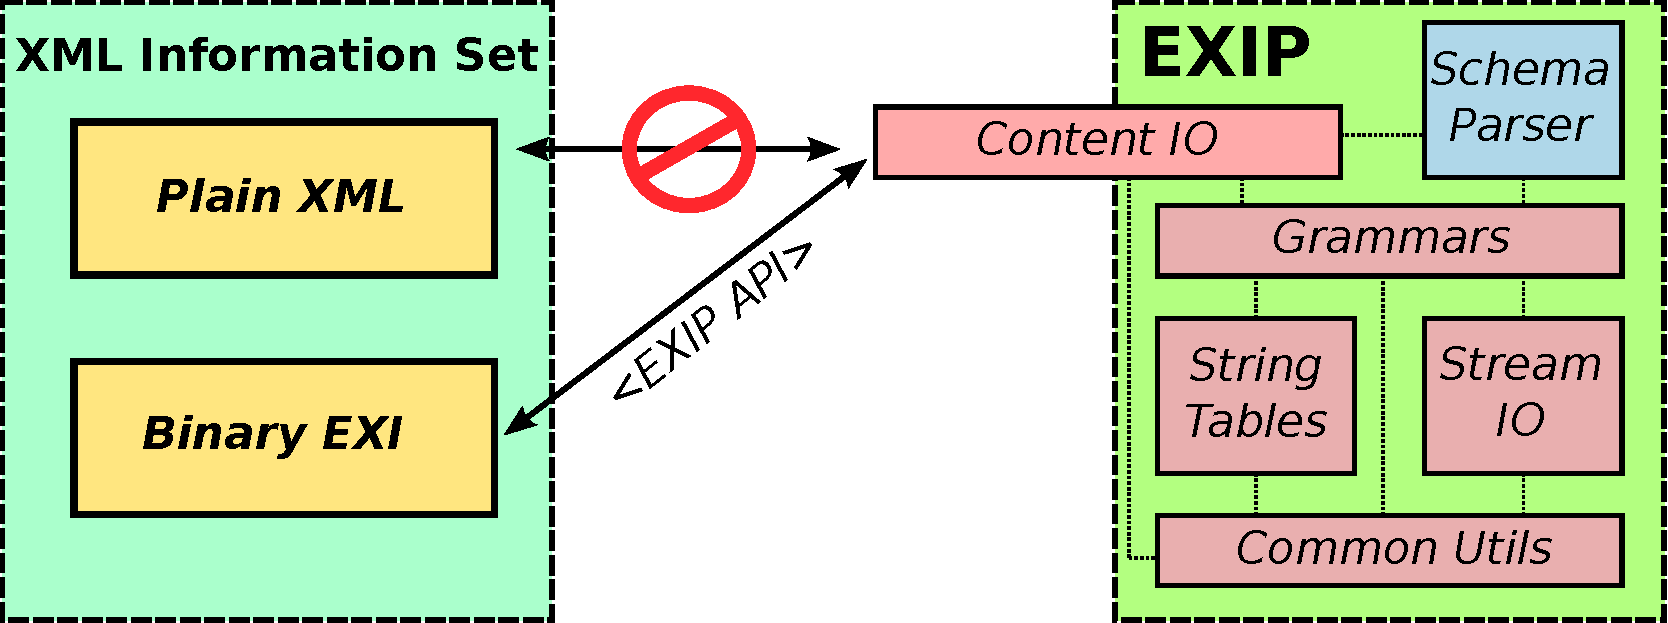
\includegraphics[width=0.90\textwidth, keepaspectratio=true]{images/EXIP-overview.pdf}
\end{center}
\caption{EXIP components}
\label{fig:EXIP-components} 
\end{figure} 

Figure \ref{fig:EXIP-components} depicts these design decisions and shows the different components of
the library. Key concept when creating the structure of the project was modularity - the functionality
is grouped and encapsulated in different components. This allows for disabling features that are not
needed directly at compile time. As an example, the Schema Parser component that is responsible for
generation the grammar structures based on XML Schema definitions is only needed if the system is
expected to dynamically handle XML schemes and hence in all other cases can be removed from the build at compile time. 

For further information and details on the EXIP API and the rational
behind it see the paper that first presents EXIP \cite{RumenKyusakov2011} (please refer to this work when 
citing information from this guide or other EXIP documentation).

\subsection{Strings in EXIP}
\label{sec:strings}

All character strings in EXIP are length prefixed. 

\subsection{Error handling and memory management}
\label{sec:errors-memory}

Some short and concise info here